\documentclass[a4paper,11pt]{jctvcdoc}

\usepackage{geometry}[2010/02/12]

\usepackage{hyperref}
\hypersetup{colorlinks=true}
\usepackage{color,soul}

\usepackage[position=bottom]{subfig}
\captionsetup[subfloat]{position=top}
\usepackage{multirow}
\usepackage{dcolumn}
\newcolumntype{.}{D{.}{.}{-1}}
\usepackage{colortbl}
\usepackage{makecell}
\usepackage{longtable}
\usepackage{array}
\usepackage{algorithm2e}

\usepackage[strings]{underscore}
\usepackage{csquotes}
\MakeOuterQuote{"}
\EnableQuotes

\newcommand\None{}
\newcommand\NotSet{}
\makeatletter
\newcommand{\Option}[1]{\ifx\optOption\@empty\gdef\optOption{#1}\else\g@addto@macro\optOption{ \\ #1}\fi}
\newcommand{\ShortOption}[1]{\ifx\optShortOption\@empty\gdef\optShortOption{#1}\else\g@addto@macro\optShortOption{ \\ #1}\fi}
\newcommand{\Default}[1]{\ifx\optDefault\@empty\gdef\optDefault{#1}\else\g@addto@macro\optDefault{ \\ #1}\fi}
\newcommand{\clearOptions}{\gdef\optOption{}\gdef\optShortOption{}\gdef\optDefault{}}
\makeatother
\newenvironment{OptionTable}[1]{%
	\footnotesize
	\def\arraystretch{1.8}
	\clearOptions
	\begin{longtable}{l<{\makecell[tl]{\optOption}}%
	                  >{\texttt\bgroup}l<{\makecell[tl]{\optShortOption}\egroup}%
	                  c<{\makecell[tc]{\optDefault}}%
	                  >{\def\arraystretch{1.0}}p{0.5\textwidth}<{\clearOptions}}
	\caption{#1} \\
	\hspace*{12em}&&\hspace*{8em}&\kill
	\hline
	 \thead{Option} &
	 \egroup\thead{Shorthand}\bgroup &
	 \thead{Default} &
	 \thead{Description} \\
	\hline
	\endfirsthead
	\caption[]{#1 (Continued)} \\
	\hspace*{12em}&&\hspace*{8em}&\kill
	\hline
	 \thead{Option} &
	 \egroup\thead{Shorthand}\bgroup &
	 \thead{Default} &
	 \thead{Description} \\
	\hline
	\endhead
	 \multicolumn{4}{r}{Continued...}\\
	 \hline
	\endfoot
	 \hline
	\endlastfoot
}{%
	\hline
	\end{longtable}
}

\newenvironment{MacroTable}[1]{%
	\footnotesize
	\def\arraystretch{1.3}
	\clearOptions
	\begin{longtable}{lcp{0.5\textwidth}}
	 \caption{#1} \\
	%\hspace*{12em}&&\hspace*{8em}&\kill
	 \hline
	  \thead{Option} &
	  \thead{Default} &
	  \thead{Description} \\
	 \hline
	\endfirsthead
	 \caption[]{#1 (Continued)} \\
	 \hline
	  \thead{Option} &
	  \thead{Default} &
	  \thead{Description} \\
	 \hline
	\endhead
	 \multicolumn{3}{r}{Continued...}\\
	 \hline
	\endfoot
	 \hline
	\endlastfoot
}{%
	\end{longtable}
}

\title{HM Software Manual}
\author{%
	Frank Bossen
	\email{bossen@docomoinnovations.com}
	\and
	David Flynn
	\email{davidf@rd.bbc.co.uk}
	\and
	Karsten S\"uhring
	\email{Karsten.Suehring@hhi.fraunhofer.de}
}

\jctvcmeeting{}
\jctvcdocnum{Software Manual}
\jctvcdocstatus{Software AHG working document}
\jctvcdocpurpose{Information}
\jctvcdocsource{AHG chairs}

\begin{document}
\maketitle
\begin{abstract}
This document is a user manual describing usage of reference software
for the HEVC project. It applies to version 8.2
of the software.
\end{abstract}

\tableofcontents
\listoftables

\section{General Information}
Reference software is being made available to provide a reference
implementation of the draft HEVC standard being developed by the Joint
Collaborative Team on Video Coding (JCT-VC) regrouping experts from
ITU-T SG 16 and ISO/IEC SC29 WG11. One of the main goals of the
reference software is to provide a basis upon which to conduct
experiments in order to determine which coding tools provide desired
coding performance. It is not meant to be a particularly efficient
implementation of anything, and one may notice its apparent
unsuitability for a particular use. It should not be construed to be a
reflection of how complex a production-quality implementation of a
future HEVC standard would be.

This document aims to provide guidance on the usage of the reference
software. It is widely suspected to be incomplete and suggestions for
improvements are welcome. Such suggestions and general inquiries may be
sent to the general JCT-VC email reflector on
\url{jct-vc@lists.rwth-aachen.de} (registration required).

\subsection*{Bug reporting}
Bugs should be reported on the issue tracker set up at
\url{http://hevc.kw.bbc.co.uk/trac/}

\section{Installation and compilation}
The software may be retrieved from one of the following SVN servers
(mirrored):
\begin{itemize}
\item \url{https://hevc.hhi.fraunhofer.de/svn/svn_HEVCSoftware/}
\item \url{svn://hevc.kw.bbc.co.uk/svn/jctvc-hm/}
\end{itemize}

Table~\ref{tab:project-files} enumerates various project files that are
provided for development environments.

\begin{table}[ht]
\footnotesize
\caption{Available project files}
\label{tab:project-files}
\centering
\begin{tabular}{ll}
\hline
 \thead{Environment} &
 \thead{Location of project file} \\
% Environment          & Location of project file \\
\hline
MS Visual Studio 8   & build/HM_vc8.sln \\
MS Visual Studio 9   & build/HM_vc9.sln \\
Xcode                & HM.xcodeproj \\
Linux                & build/linux/makefile \\
\hline
\end{tabular}
\end{table}

%%%%
%%%%
%%%%
\section{Using the encoder}
\begin{verbatim}
TAppEncoder 	[-h] [-c config.cfg] [--parameter=value]
\end{verbatim}

\begin{table}[ht]
\footnotesize
\centering
\begin{tabular}{lp{0.5\textwidth}}
\hline
 \thead{Option} &
 \thead{Description} \\
\hline
\texttt{-h} & Prints parameter usage. \\
\texttt{-c} & Defines configuration file to use.  Multiple configuration files
     may be used with repeated --c options. \\
\texttt{--}\emph{parameter}\texttt{=}\emph{value}
    & Assigns value to a given parameter as further described below.
      Some parameters are also supported by shorthand
      "--\em{opt}~\emph{value}".\\
\hline
\end{tabular}
\end{table}

Sample configuration files are provided in the cfg/ folder.

\subsection{GOP structure table}
\label{sec:gop-structure}
Defines the cyclic GOP structure that will be used repeatedly
throughout the sequence. The table should contain GOPSize lines,
named Frame1, Frame2, etc. The frames are listed in decoding
order, so Frame1 is the first frame in decoding order, Frame2 is
the second and so on. Among other things, the table specifies all
reference pictures kept by the decoder for each frame. This
includes pictures that are used for reference for the current
picture as well as pictures that will be used for reference in
the future. The encoder will not automatically calculate what
pictures that has to be kept for future references, they have to
be specified. Note that some specified reference frames for
pictures encoded in the very first GOP after an IDR frame might
not be available. This is handled automatically by the encoder,
so the reference pictures can be given in the GOP structure table
as if there were infinitely many identical GOPs before the
current one. Each line in the table contains the parameters used
for the corresponding frame, separated by whitespace:

\begin{itemize}
\item[]\textbf{Type}: Slice type, can be either I, P or B.

\item[]\textbf{POC}: Display order of the frame within a GOP, ranging
from 1 to GOPSize.

\item[]\textbf{QPOffset}: QP offset is added to the QP parameter to set
the final QP value to use for this frame.

\item[]\textbf{QPFactor}: Weight used during rate distortion
optimization. Higher values mean lower quality and less bits. Typical
range is between
0.3 and 1.

\item[]\textbf{temporal_id}: Temporal layer of the frame. A frame cannot
predict from a frame with a higher temporal id. If a frame with higher
temporal IDs is listed among a frame's reference pictures, it is
not used, but is kept for possible use in future frames.

\item[]\textbf{num_ref_pics_active}: Size of reference picture lists L0
and L1, indicating how many reference pictures in each direction that
are used during coding.

\item[]\textbf{num_ref_pics}: The number of reference pictures kept for
this frame.  This includes pictures that are used for reference for the
current picture as well as pictures that will be used for reference in
the future.

\item[]\textbf{reference_pictures}: A space-separated list of
num_ref_pics integers, specifying the POC of the reference pictures
kept, relative the POC of the current frame. The picture list shall be
ordered, first with negative numbers from largest to smallest, followed
by positive numbers from smallest to largest (e.g. \verb|-1 -3 -5 1 3|).
Note that any pictures not supplied in this list will be discarded and
therefore not available as reference pictures later.

\item[]\textbf{predict}: Defines the value of the syntax element
inter_ref_pic_set_prediction_flag. A value of 0 indicates that the
reference picture set is encoded without inter RPS prediction and the
subsequent parameters deltaRIdx$-1$, deltaRPS, num_ref_idcs and
Reference_idcs are ignored and do not need to be present. A value of 1
indicates that the reference picture set is encoded with inter
prediction RPS using the subsequent parameters deltaRIdx$-1$, deltaRPS,
num_ref_idcs and Reference_idcs in the line. A value of 2 indicates that
the reference picture set is encoded with inter RPS but only the
deltaRIdx$-1$ parameters is needed. The deltaRPS, num_ref_idcs and
Reference_idcs values are automatically derived by the encoder based on
the POC and refPic values of the current line and the RPS pointed to by
the deltaRIdx$-1$ parameters.

\item[]\textbf{deltaRIdx$-1$}: The difference between the index of the
curent RPS and the predictor RPS minus 1.

\item[]\textbf{deltaRPS}: The difference between the POC of the
predictor RPS and POC the current RPS.

\item[]\textbf{num_ref_idcs}: The number of ref_idcs to encode for the
current RPS.  The value is equal to the value of  num_ref_pics of the
predictor RPS plus 1.

\item[]\textbf{reference_idcs}: A space-separated list of num_ref_idcs
integers, specifying the ref idcs of the inter RPS prediction. The value
of ref_idcs may be 0, 1 or 2 indicating that the reference picture is a
reference picture used by the current picture, a reference picture used
for future picture or not a reference picture anymore, respectively. The
first num_ref_pics of ref_idcs correspond to the Reference pictures in
the predictor RPS. The last ref_idcs corresponds to the predictor
picture.
\end{itemize}

For example, consider the coding structure of Figure~\ref{fig:gop-example}.
This coding structure is of size 4. The pictures are listed in decoding
order. Frame1 shall therefore describe picture with $\textrm{POC}=4$. It
references picture 0, and therefore has $-4$ as a reference picture.
Similarly, Frame2 has a POC of 2, and since it references pictures 0 and
4, its reference pictures are listed as \verb|-2 2|. Frame3 is a special
case: even though it only references pictures with POC 0 and 2, it also
needs to include the picture with POC 4, which must be kept in order to
be used as a reference picture in the future. The reference picture list
for Frame3 therefore becomes \verb|-1 1 3|. Frame4 has a POC of 3 and
its list of reference pictures is \verb|-1 1|.

\begin{figure}[h]
\caption{A GOP structure}
\label{fig:gop-example}
\centering
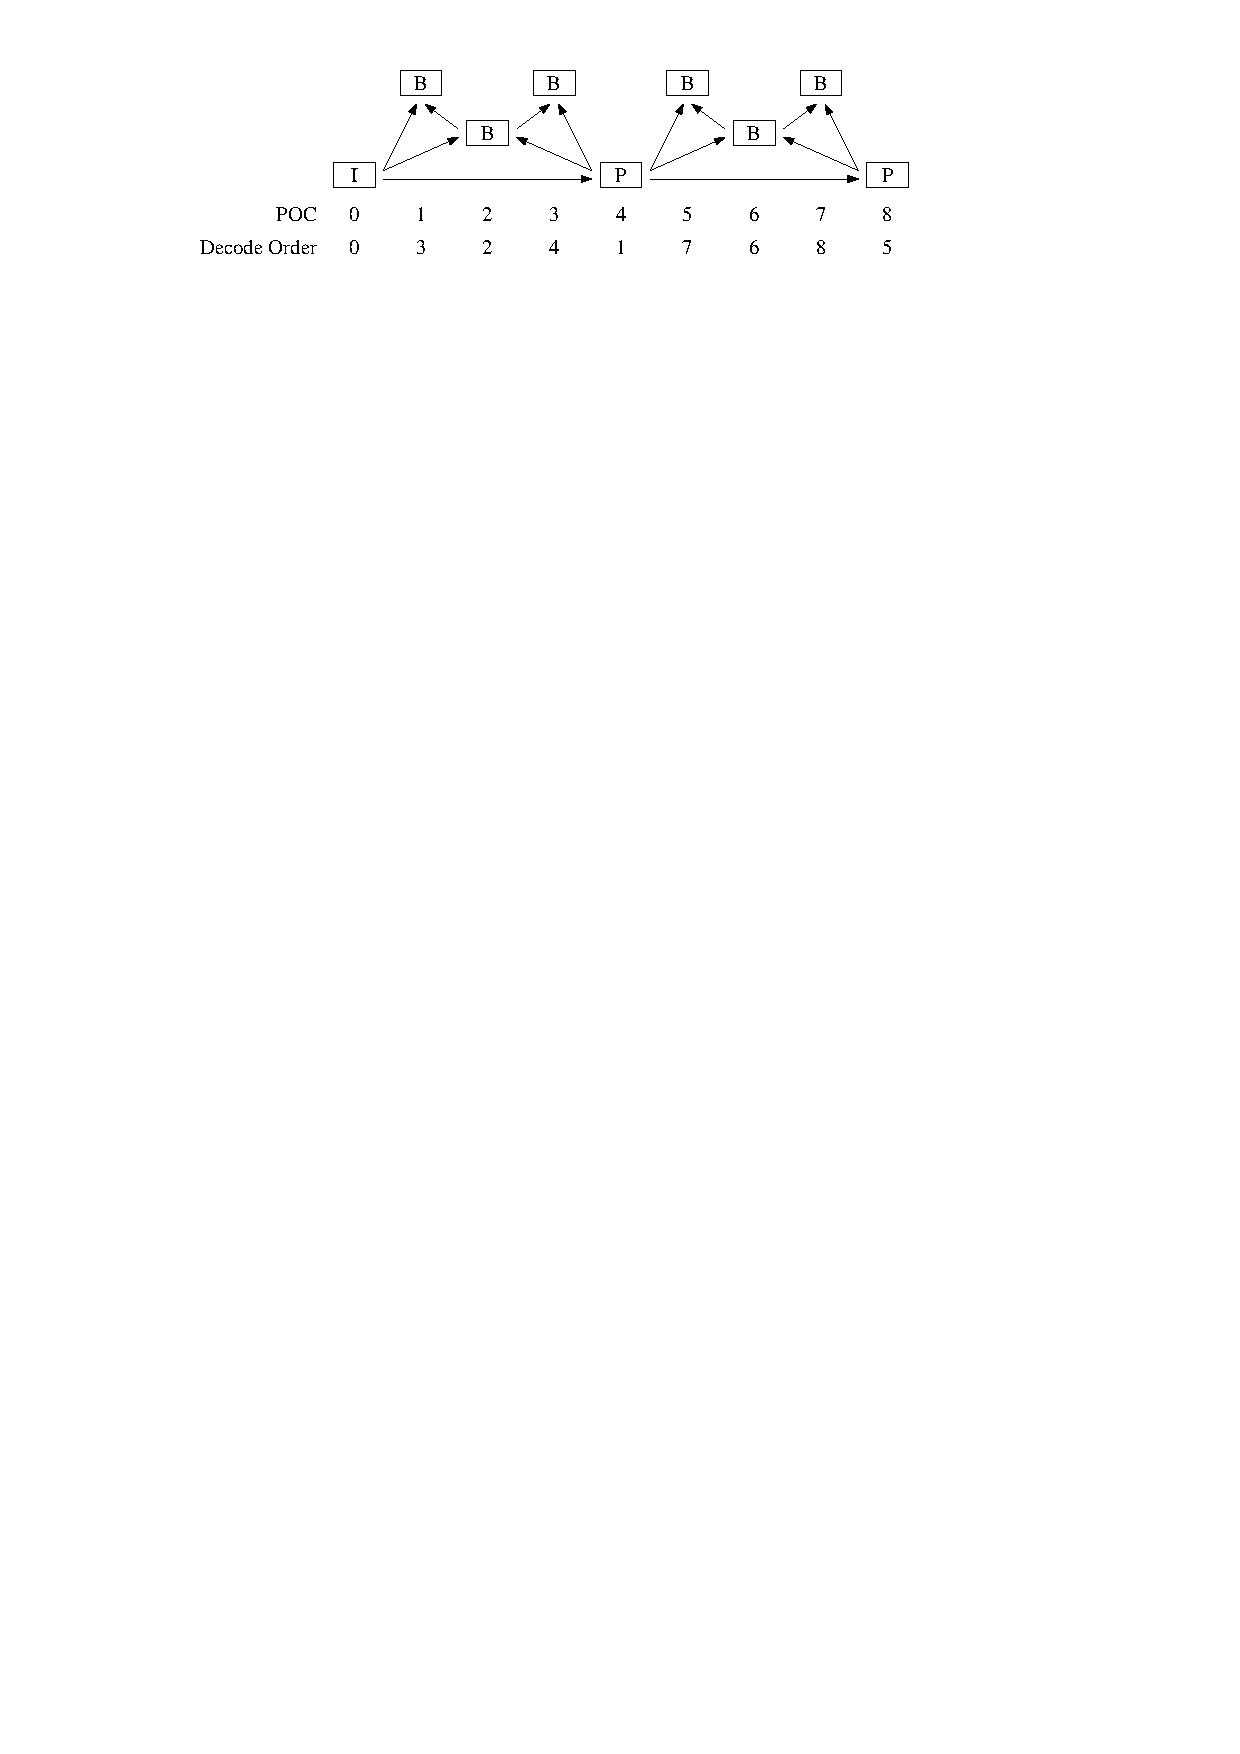
\includegraphics[width=0.7\textwidth]{gop-structure-example}
\end{figure}

Inter RPS prediction may be used for Frame2, Frame3 and Frame4, hence
the predict parameter is set to 1 for these frames. Frame2 uses Frame1
as the predictor hence the deltaRIdx$-1$ is 0.  Similarly for Frame3 and
Frame4 which use Frame2 and Frame3 as predictors, respectively. The
deltaRPS is equal to the POC of the predictor minus the POC of the
current picture, therefore the deltaRPS for Frame2 is $4 -2 = 2$, for
Frame3 is $2 - 1 = 1$ and for Frame4 is $1 - 3 = -2$.

In Frame2, reference pictures with POC 0 and 2 are used, so the
reference idcs for Frame2 are \verb|1 1| indicating that the reference
picture, $-4$, in Frame1 is still a reference picture in Frame2 and
Frame1 is also a reference picture in Frame2. The reference idcs for
Frame3 are \verb|1 1 1|. The first and second “1”s indicating that
the reference pictures "$-2$ $2$" in Frame2 are still reference pictures in
Frame3 and the last “1” indicating that Frame2 is also a reference
picture in Frame3. In Frame 4, the reference idcs are \verb|0 1 1 0|.
The first “0” indicates that the reference pictures “-1” in Frame 3 is
no longer a reference picture in Frame4. The next two “1”s indicate that
the reference pictures “$1$ $3$” are now reference pictures of Frame4.
The final “0” indicates that Frame3 is not a reference picture.

In order to specify this to the encoder, the parameters in
Table~\ref{tab:gop-example} could be used.

\begin{table}[ht]
\footnotesize
\caption{GOP structure example}
\label{tab:gop-example}
\centering
\begin{tabular}{lrrrr}
\hline
 \thead{} &
 \thead{Frame1} &
 \thead{Frame2} &
 \thead{Frame3} &
 \thead{Frame4} \\
\hline
Type                &   P  &    B   &      B   &       B \\
POC                 &   4  &    2   &      1   &       3 \\
QPoffset            &   1  &    2   &      3   &       3 \\
QPfactor            & 0.5  &  0.5   &    0.5   &     0.5 \\
temporal_id         &   0  &    1   &      2   &       2 \\
num_ref_pics_active &   1  &    1   &      1   &       1 \\
num_ref_pics        &   1  &    2   &      3   &       2 \\
reference_pictures  & $-$4 & $-$2 2 & $-$1 1 3 &  $-$1 1 \\
predict             &   0  &    1   &      1   &       1 \\
deltaRIdx$-$1       &      &    0   &      0   &       0 \\
deltaRPS            &      &    2   &      1   &    $-$2 \\
num_ref_idcs        &      &    2   &      3   &       4 \\
reference_idcs      &      &  1 1   &  1 1 1   & 0 1 1 0 \\
\hline
\end{tabular}
\end{table}

Here, the frames used for prediction have been given higher
quality by assigning a lower QP offset. Also, the non-reference
frames have been marked as belonging to a higher temporal layer,
to make it possible to decode only every other frame. Note: each
line should contain information for one frame, so this
configuration would be specified as:

\begin{verbatim}
Frame1: P 4 1 0.5 0 1 1 -4 0
Frame2: B 2 2 0.5 1 1 2 -2 2 1 0 2 2 1 1
Frame3: B 1 3 0.5 2 1 3 -1 1 3 1 0 1 3 1 1 1
Frame4: B 3 3 0.5 2 1 2 -1 1 1 0 -2 4 0 1 1 0
\end{verbatim}

The values of deltaRIdx$-1$, deltaRPS, num_ref_idcs and reference
idcs of Frame$K$ can be derived from the POC value of Frame$_K$ and
the POC, num_ref_pics and reference_pictures values of Frame$_M$, where
$K$ is the index of the RPS to be inter coded and the $M$ is the
index of the reference RPS, as follows.

\setlength{\algomargin}{2em}
\begin{algorithm}[h]
\SetKwData{deltaRIdx}{deltaRIdx}
\SetKwData{deltaRPS}{deltaRPS}
\SetKwData{numrefidcs}{num_ref_idcs}
\SetKwData{numrefpics}{num_ref_pics}
\SetKwData{referencepictures}{reference_pictures}
\SetKwData{referenceidcs}{reference_idcs}
\SetKwData{POC}{POC}

$\deltaRIdx_K - 1  \leftarrow  K - M - 1$ \;
$\deltaRPS_K       \leftarrow  \POC_M - \POC_K$ \;
$\numrefidcs_K     \leftarrow  \numrefpics_M + 1$ \;

\For{$j \leftarrow 0$ \KwTo $\numrefpics_M$}{
	\For{$i \leftarrow 0$ \KwTo $\numrefidcs_K$}{
		\eIf{$\referencepictures_{M,j} + \deltaRPS_K == \referencepictures_{K,i}$}{
			\lIf{$\referencepictures_{K,i}$ is used by the current frame}{
				$\referenceidcs_{K,j} = 1$} \;
			\lElse{$\referenceidcs_{K,j} = 2$} \;
		}{
			$\referenceidcs_K[j] = 0$ \;
		}
	}
}

\tcc{$\referencepictures_{M,\numrefpics_M}$ does not exist and is assumed to be 0}
\end{algorithm}

Note: The above (automatic) generation of the inter RPS parameter
values has been integrated into the encoder, and is activated by
the value of predict $= 2$ followed by the value of deltaRIdx$-1$,
only, as described above.



%%%%
%%%%
%%%%
\newgeometry{tmargin=1.6cm,lmargin=1cm,rmargin=1cm,bmargin=1in,nohead}
\subsection{Encoder parameters}

%%
%% File, I/O and source parameters
%%
\begin{OptionTable}{File, I/O and source parameters}
\Option{InputFile} &
\ShortOption{-i} &
\Default{\NotSet} &
Specifies the input video file.

Video data must be in a raw 4:2:0 planar format (Y$'$CbCr).

Note: When the bit depth of samples is larger than 8, each sample is encoded in
2 bytes (little endian, LSB-justified).
\\

\Option{BitstreamFile} &
\ShortOption{-b} &
\Default{\NotSet} &
Specifies the output coded bit stream file.
\\

\Option{ReconFile} &
\ShortOption{-o} &
\Default{\NotSet} &
Specifies the output locally reconstructed video file.
\\

\Option{SourceWidth}%
\Option{SourceHeight} &
\ShortOption{-wdt}%
\ShortOption{-hgt} &
\Default{0}%
\Default{0} &
Specifies the width and height of the input video in luma samples.
\\

\Option{InputBitDepth} &
\ShortOption{\None} &
\Default{8} &
Specifies the bit depth of the input video.
\\

\Option{InternalBitDepth} &
\ShortOption{\None} &
\Default{0 \\ (InputBitDepth)} &
Specifies the bit depth used for coding.

If the input video is a different bit depth to InternalBitDepth, it is
automatically converted by:
\begin{displaymath}
\left\lfloor
 \frac{\mathrm{Pel} * 2^{\mathrm{InternalBitDepth}}}{
     2^{\mathrm{InputBitDepth}}}
\right\rfloor
\end{displaymath}

Note: The effect of this option is as if the input video is externally
converted to the InternalBitDepth and then coded with this value as
InputBitDepth.  The codec has no notion of two different bit depths.
\\

\Option{OutputBitDepth} &
\ShortOption{\None} &
\Default{0 \\ (InternalBitDepth)} &
Specifies the bit depth of the output locally reconstructed video file.

Note: This option has no effect on the decoding process.
\\

\Option{CroppingMode} &
\ShortOption{\None} &
\Default{0} &
Specifies the cropping/padding parameters to be applied to the input
video. The following modes are available:
\par
\begin{tabular}{cp{0.45\textwidth}}
0 & No cropping / padding \\
1 & Automatic padding to the next minimum CU size \\
2 & Padding according to parameters HorizontalPadding and VerticalPadding \\
3 & Cropping according to parameters CropLeft, CropRight, CropTop and
    CropBottom \\
\end{tabular}
\\

\Option{HorizontalPadding}%
\Option{VerticalPadding} &
\ShortOption{-pdx}%
\ShortOption{-pdy} &
\Default{0} &
Specifies the horizontal and vertical padding to be applied to the input
video in luma samples.  Must be a multiple of the chroma resolution
(e.g. a multiple of two for 4:2:0).
\\

\Option{CropLeft}%
\Option{CropRight}%
\Option{CropTop}%
\Option{CropBottom} &
\ShortOption{\None} &
\Default{0} &
Specifies the horizontal and vertical cropping to be applied to the
input video in luma samples.  Must be a multiple of the chroma
resolution (e.g. a multiple of two for 4:2:0).
\\

\Option{FrameRate} &
\ShortOption{-fr} &
\Default{0} &
Specifies the frame rate of the input video.

Note: This option only affects the reported bit rates.
\\

\Option{FrameSkip} &
\ShortOption{-fs} &
\Default{0} &
Specifies a number of frames to skip at beginning of input video file.
\\

\Option{FramesToBeEncoded} &
\ShortOption{-f} &
\Default{0 \\ (all)} &
Specifies the number of frames to be encoded.
\\
\end{OptionTable}


%%
%% Unit definition parameters
%%
\begin{OptionTable}{Unit definition parameters}
\Option{MaxCUWidth} &
\ShortOption{\None} &
\Default{64} &
Defines the maximum CU width.
\\

\Option{MaxCUHeight} &
\ShortOption{\None} &
\Default{64} &
Defines the maximum CU height.
\\

\Option{MaxCUSize} &
\ShortOption{\None} &
\Default{64} &
Defines the maximum CU size.
\\

\Option{MaxPartitionDepth} &
\ShortOption{-h} &
\Default{4} &
Defines the depth of the CU tree.
\\

\Option{QuadtreeTULog2MaxSize} &
\ShortOption{\None} &
\Default{6 \\ ($= \mathrm{log}_2(64)$)} &
Defines the Maximum TU size in logarithm base 2.
\\

\Option{QuadtreeTULog2MinSize} &
\ShortOption{\None} &
\Default{2 \\ ($= \mathrm{log}_2(4)$)} &
Defines the Minimum TU size in logarithm base 2.
\\

\Option{QuadtreeTUMaxDepthIntra} &
\ShortOption{\None} &
\Default{1} &
Defines the depth of the TU tree for intra CUs.
\\

\Option{QuadtreeTUMaxDepthInter} &
\ShortOption{\None} &
\Default{2} &
Defines the depth of the TU tree for inter CUs.
\\
\end{OptionTable}


%%
%% Coding structure parameters
%%
\begin{OptionTable}{Coding structure parameters}
\Option{IntraPeriod} &
\ShortOption{-ip} &
\Default{$-1$} &
Specifies the intra frame period.
A value of $-1$ implies an infinite period.
\\

\Option{DecodingRefreshType} &
\ShortOption{-dr} &
\Default{0} &
Specifies the type of decoding refresh to apply at the intra frame period
picture.
\par
\begin{tabular}{cp{0.45\textwidth}}
0 & Applies an I picture (not a clean random access point). \\
1 & Applies a non-IDR clean random access point (open GOP). \\
2 & Applies an IDR random access point (closed GOP). \\
\end{tabular}
\\

\Option{GOPSize} &
\ShortOption{-g} &
\Default{1} &
Specifies the size of the cyclic GOP structure.
\\

\Option{Frame\emph{N}} &
\ShortOption{\None} &
\Default{\NotSet} &
Multiple options that define the cyclic GOP structure that will be used
repeatedly throughout the sequence.  The table should contain GOPSize
elements.
\par
See section~\ref{sec:gop-structure} for further details.
\\

\Option{ListCombination} &
\ShortOption{-lc} &
\Default{true} &
Enables or disables the use of the combined reference list for uni-prediction
in B-slices.
\par
\begin{tabular}{cp{0.45\textwidth}}
  0 & Reference list~0 and reference list~1 are identical and reference
      list~0 is used as the combined reference list. \\
  1 & The combined reference list is derived from reference list~0 and
      reference list~1. \\
\end{tabular}
NB: LComb can only be 0 in low delay coding (more precisely, when list 0
and list 1 are the same)
\\
\end{OptionTable}


%%
%% Motion estimation parameters
%%
\begin{OptionTable}{Motion estimation parameters}
\Option{FastSearch} &
\ShortOption{\None} &
\Default{true} &
Enables or disables the use of a fast motion search.
\par
\begin{tabular}{cp{0.45\textwidth}}
 0 & Full search method \\
 1 & Fast search method \\
\end{tabular}
\\

\Option{SearchRange} &
\ShortOption{-sr} &
\Default{96} &
Specifies the search range used for motion estimation.

Note: the search range is defined around a predictor. Motion vectors
derived by the motion estimation may thus have values larger than the
search range.
\\

\Option{BipredSearchRange} &
\ShortOption{\None} &
\Default{4} &
Specifies the search range used for bi-prediction refinement in motion
estimation.
\\

\Option{HadamardME} &
\ShortOption{\None} &
\Default{true} &
Enables or disables the use of the Hadamard transform in fractional-pel motion
estimation.
\par
\begin{tabular}{cp{0.45\textwidth}}
 0 & SAD for cost estimation \\
 1 & Hadamard for cost estimation \\
\end{tabular}
\\

\Option{ASR} &
\ShortOption{\None} &
\Default{false} &
Enables or disables the use of adaptive search ranges, where the motion
search range is dynamically adjusted according to the POC difference
between the current and the reference pictures.
\begin{displaymath}
\resizebox{\hsize}{!}{$
\mathrm{SearchRange}’ = \mathrm{Round}\left(
                          \mathrm{SearchRange}
                          * \mathrm{ADAPT\_SR\_SCALE}
                          * \frac{\mathrm{abs}(
                                 \mathrm{POCcur} - \mathrm{POCref} )}{
                                 \mathrm{RateGOPSize}}\right)
$}
\end{displaymath}
\\
\end{OptionTable}


%%
%% Mode decision parameters
%%
\begin{OptionTable}{Mode decision parameters}
\Option{LambdaModifier$N$} &
\ShortOption{-LM$N$} &
\Default{1.0} &
Specifies a value that is multiplied with the Lagrange multiplier
$\lambda$, for use in the rate-distortion optimised cost calculation
when encoding temporal layer~$N$.
\par
$N$ may be in the range 0--7.
\\

\Option{FEN} &
\ShortOption{\None} &
\Default{false} &
Enables or disables the use of fast encoder mode.  When enabled,
the following occurs:
\begin{itemize}
\item In the SAD computation for blocks having size larger than 8, only
      the lines of even rows in the block are considered.
\item The number of iterations used in the bi-directional motion vector
      refinement in the motion estimation process is reduced from 4 to 1.
\end{itemize}
\\

\Option{FDM} &
\ShortOption{\None} &
\Default{true} &
Enables or disables the use of fast encoder decisions for 2Nx2N merge
mode.  When enabled, the RD cost for the merge mode of the current
candidate is not evaluated if the merge skip mode was the best merge
mode for one of the previous candidates.
\\
\end{OptionTable}

%%
%% Quantization parameters
%%
\begin{OptionTable}{Quantization parameters}
\Option{QP} &
\ShortOption{-q} &
\Default{30.0} &
Specifies the base value of the quantization parameter.
\\

\Option{CbQpOffset}%
\Option{CrQpOffset} &
\ShortOption{-cbqpofs}%
\ShortOption{-crqpofs} &
\Default{0}%
\Default{0} &
Global offset to apply to the luma QP to derive the QP of Cb and Cr
respectively.  These options correspond to the values of cb_qp_offset
and cr_qp_offset, that are transmitted in the PPS.  Valid values are in
the range $[-12, 12]$.
\\

\Option{MaxCuDQPDepth} &
\ShortOption{\None} &
\Default{0} &
Defines maximum depth of a minimum CuDQP for sub-LCU-level delta QP.
MaxCuDQPDepth shall be greater than or equal to SliceGranularity.
\\

\Option{RDOQ} &
\ShortOption{\None} &
\Default{true} &
Enables or disables rate-distortion-optimized quantization.
\\

\Option{DeltaQpRD} &
\ShortOption{-dqr} &
\Default{0} &
Specifies the maximum QP offset at slice level for multi-pass slice
encoding.  When encoding, each slice is tested multiple times by using
slice QP values in the range $[-\mathrm{DeltaQpRD}, \mathrm{DeptaQpRD}]$,
and the best QP value is chosen as the slice QP.
\\

\Option{MaxDeltaQP} &
\ShortOption{-d} &
\Default{0} &
Specifies the maximum QP offset at the largest coding unit level for
the block-level adaptive QP assignment scheme. In the encoder, each
largest coding unit is tested multiple times by using the QP values in
the range $[-\mathrm{MaxDeltaQP}, \mathrm{MaxDeltaQP}]$, and the best QP
value is chosen as the QP value of the largest coding unit.
\\

\Option{dQPFile} &
\ShortOption{-m} &
\Default{\NotSet} &
Specifies a file containing a list of QP deltas. The $n$-th line
(where $n$ is 0 for the first line) of this file corresponds to the QP
value delta for the picture with POC value $n$.
\\

\Option{AdaptiveQpSelection} &
\ShortOption{-aqps} &
\Default{false} &
Specifies whether QP values for non-I frames will be calculated on the
fly based on statistics of previously coded frames.
\\
\Option{RecalculateQPAccordingToLambda} &
\ShortOption{\None} &
\Default{false} &
Recalculate QP values according to lambda values. Do not suggest to be enabled in all intra case.
\\
\end{OptionTable}



%%
%% Entropy coding parameters
%%
\begin{OptionTable}{Entropy coding parameters}
\Option{SBACRD} &
\ShortOption{\None} &
\Default{true} &
Enables or disables the use of bit counts from arithmetic coder in
rate-distortion decisions.
\\
\end{OptionTable}


%%
%% Slice coding parameters
%%
\begin{OptionTable}{Slice coding parameters}
%\Option{SliceGranularity} &
%\ShortOption{\None} &
%\Default{0} &
%Determines the depth in an LCU at which slices may begin and end.
%\par
%\begin{tabular}{cp{0.45\textwidth}}
% 0   & Slice addresses are LCU aligned \\
% $1 \leq n \leq 3$
%     & Slice start addresses are aligned to CUs at depth $n$ \\
%\end{tabular}
%
%Note: The smallest permissible alignment is 16x16 CUs.
%Values of $n$ must satisfy this constraint, for example, with a 64x64
%LCU, $n$ must be less than or equal to 2.
%\\

\Option{SliceMode} &
\ShortOption{\None} &
\Default{0} &
Controls the slice partitioning method in conjunction with
SliceArgument.
\par
\begin{tabular}{cp{0.45\textwidth}}
 0 & Single slice \\
 1 & Maximum number of CUs (at a depth of SliceGranuarity) per slice \\
 2 & Maximum number of bytes per slice \\
\end{tabular}
\\

\Option{SliceArgument} &
\ShortOption{\None} &
\Default{\NotSet} &
Specifies the maximum number of CUs or bytes in a slice depending on the
SliceMode setting.
\\

\Option{EntropySliceMode} &
\ShortOption{\None} &
\Default{0} &
Enables entropy slice coding. When set to 1, the parameter SliceArgument
will specify the maximum number of CUs in a slice. When set to 2, the
parameter SliceArgument will specify the number of bytes (LCEC) or bins
(CABAC) in a slice.
\\

\Option{EntropySliceArgument} &
\ShortOption{\None} &
\Default{\NotSet} &
Defines the maximum number of CUs or bytes/bins in an entropy slice
depending on the SliceMode setting.
\\

\Option{WaveFrontSynchro} &
\ShortOption{\None} &
\Default{false} &
Enables the use of specific CABAC probabilities synchronization at the
beginning of each line of CTBs in order to produce a bitstream that can
be encoded or decoded using one or more cores.
\\

\Option{NumTileColumnsMinus1}%
\Option{NumTileRowsMinus1} &
\ShortOption{\None} &
\Default{0} &
Specifies the tile based picture partitioning geometry as
$\mathrm{NumTileColumnsMinus1} + 1 \times \mathrm{NumTileRowsMinus1} + 1$
columns and rows.
\\

\Option{UniformSpacingIdc} &
\ShortOption{\None} &
\Default{0} &
Controls the mode used to determine per row and column tile sizes.
\par
\begin{tabular}{cp{0.45\textwidth}}
 0 & Each tile column width and tile row height is explicitly set
     by ColumnWidthArray and RowHeightArray respectively \\
 1 & Tile columns and tile rows are uniformly spaced. \\
\end{tabular}
\\

\Option{ColumnWidthArray}%
\Option{RowHeightArray} &
\ShortOption{\None} &
\Default{\NotSet} &
Specifies a space or comma separated list of widths and heights,
respectively, of each tile column or tile row.  The first value in the
list corresponds to the leftmost tile column or topmost tile row.
\\
\end{OptionTable}



%%
%% Deblocking filter parameters
%%
\begin{OptionTable}{Deblocking filter parameters}
\Option{LoopFilterDisable} &
\ShortOption{\None} &
\Default{false} &
Enables or disables the in-loop deblocking filter.
\\

\Option{LFCrossSliceBoundaryFlag} &
\ShortOption{\None} &
\Default{true} &
Enables or disables the use of in-loop filtering across slice
boundaries.
\\

\Option{DeblockingFilterControlPresent}&
\ShortOption{\None}&
\Default{false}&
Enables or disables the presence of the deblocking filter control
parameters in the picture parameter set and in the slice header.
When disabled, the default deblocking filter parameters are used.
\\
\end{OptionTable}



%%
%% Coding tools parameters
%%
\begin{OptionTable}{Coding tools parameters}
%\Option{ALF} &
%\ShortOption{\None} &
%\Default{true} &
%Enables or disables the adaptive loop filter.
%\\

%\Option{ALFLowLatencyEncode} &
%\ShortOption{\None} &
%\Default{false} &
%Specifies the operating mode (low latency or high efficiency) of the
%adaptive loop filter.
%\\

\Option{SAO} &
\ShortOption{\None} &
\Default{true} &
Enables or disables the sample adaptive offset (SAO) filter.
\\

\Option{SAOLcuBoundary} &
\ShortOption{\None} &
\Default{false} &
Enables or disables SAO parameter estimation using non-deblocked pixels
for LCU bottom and right boundary areas.
\\

%\Option{LMChroma} &
%\ShortOption{\None} &
%\Default{true} &
%Enables or disables the intra chroma-from-luma prediction mode.
%\\

%\Option{NSQT} &
%\ShortOption{\None} &
%\Default{true} &
%Enables or disables the non-square quadtree transform.
%\\

\Option{ConstrainedIntraPred} &
\ShortOption{\None} &
\Default{false} &
Enables or disables constrained intra prediction.  Constrained intra
prediction only permits samples from intra blocks in the same slice as the
current block to be used for intra prediction.
\\

\Option{TransquantBypassEnableFlag} &
\ShortOption{\None} &
\Default{false} &
Enables or disables the ability to bypass the transform,
quantization and filtering stages at CU level.
This option corresponds to the value of
transquant_bypass_enable_flag that is transmitted in the PPS.

See CUTransquantBypassFlagValue for further details.
\\

\Option{CUTransquantBypassFlagValue} &
\ShortOption{\None} &
\Default{0} &
Controls the per CU transformation, quantization and filtering
mode decision.
This option corresponds to the value of the per CU cu_transquant_bypass_flag.
\par
\begin{tabular}{cp{0.45\textwidth}}
 0 & Bypass is not performed on any CU \\
 1 & Bypass is performed on all CUs \\
\end{tabular}

This option has no effect if TransquantBypassEnableFlag is disabled.
\\

\Option{PCMEnabledFlag} &
\ShortOption{\None} &
\Default{false} &
Enables or disables the use of PCM.
\\

\Option{PCMLog2MaxSize} &
\ShortOption{\None} &
\Default{5 \\ ($= \mathrm{log}_2(32)$)} &
Specifies log2 of the maximum PCM block size. When PCM is enabled, the
PCM mode is available for 2Nx2N intra PUs smaller than or equal to the
specified maximum PCM block size
\\

\Option{PCMLog2MinSize} &
\ShortOption{\None} &
\Default{3} &
Specifies log2 of the minimum PCM block size. When PCM is enabled, the
PCM mode is available for 2Nx2N intra PUs larger than or equal to the
specified minimum PCM block size.
\par
When larger than PCMLog2MaxSize, PCM mode is not used.
\\

\Option{PCMInputBitDepthFlag} &
\ShortOption{\None} &
\Default{1} &
If enabled specifies that PCM sample bit-depth is set equal to
InputBitDepth. Otherwise, it specifies that PCM sample bit-depth is set
equal to InternalBitDepth.
\\

\Option{PCMFilterDisableFlag} &
\ShortOption{\None} &
\Default{false} &
If enabled specifies that loop-filtering on reconstructed samples of PCM
blocks is skipped. Otherwise, it specifies that loop-filtering on
reconstructed samples of PCM blocks is not skipped.
% 0 = (loop-filtering is not skipped for PCM samples).
\\

\Option{weighted_pred_flag} &
\ShortOption{-wpP} &
\Default{false} &
Controls the use of weighted prediction in P slices.
\\

\Option{weighted_bipred_idc} &
\ShortOption{-wpB} &
\Default{0} &
Controls the use of weighted prediction in B slices.
\par
\begin{tabular}{cp{0.45\textwidth}}
0 & Disabled \\
1 & Explicit weighted prediction \\
2 & Implicit weighted prediction \\
\end{tabular}
\\

\Option{SignHideFlag} &
\ShortOption{-SBH} &
\Default{true} &
If enabled specifies that for each 4x4 coefficient group for which the
number of coefficients between the first nonzero coefficient and the
last nonzero coefficient along the scanning line exceeds 4, the sign bit
of the first nonzero coefficient will not be directly transmitted in the
bitstream, but may be inferred from the parity of the sum of all nonzero
coefficients in the current coefficient group.
\\

\Option{TMVPMode} &
\ShortOption{\None} &
\Default{1} &
Controls the temporal motion vector prediction mode.
\par
\begin{tabular}{cp{0.45\textwidth}}
  0 & Disabled for all slices. \\
  1 & Enabled for all slices. \\
  2 & Disabled only for the first picture of each GOPSize. \\
\end{tabular}
\\

\Option{TransformSkip} &
\ShortOption{\None} &
\Default{false} &
Enables or disables transform-skipping mode decision for 4x4 TUs
\footnote{Enables transform_skip_enabled and per 4x4 TU tests}.
\\

\Option{TransformSkipFast} &
\ShortOption{\None} &
\Default{false} &
Enables or disables reduced testing of the transform-skipping mode
decision for chroma TUs.  When enabled, no RDO search is performed for
chroma TUs, instead they are transform-skipped if the four corresponding
luma TUs are also skipped.
\par
This option has no effect if TransformSkip is disabled.
\\
\end{OptionTable}

%%
%% VUI parameters
%%
\begin{OptionTable}{VUI parameters}
\Option{VuiParametersPresent} &
\ShortOption{-vui} &
\Default{false} &
Enable generation of vui_parameters().
\\
\Option{AspectRatioInfoPresent} &
\ShortOption{} &
\Default{false} &
Signals whether aspect_ratio_idc is present.
\\
\Option{AspectRatioIdc} &
\ShortOption{} &
\Default{0} &
aspect_ratio_idc
\\
\Option{SarWidth} &
\ShortOption{} &
\Default{0} &
Specifies the horizontal size of the sample aspect ratio.
\\
\Option{SarHeight} &
\ShortOption{} &
\Default{0} &
Specifies the vertical size of the sample aspect ratio.
\\
\Option{OverscanInfoPresent} &
\ShortOption{} &
\Default{false} &
Signals whether overscan_info_present_flag is present.
\\
\Option{OverscanAppropriate} &
\ShortOption{} &
\Default{false} &
Indicates whether cropped decoded pictures are suitable for display using overscan.
\par
\begin{tabular}{cp{0.45\textwidth}}
  0 & Indicates that the decoded pictures should not be displayed using overscan. \\
  1 & Indicates that the decoded pictures may be displayed using overscan. \\
\end{tabular}
\\
\Option{VideoSignalTypePresent} &
\ShortOption{} &
\Default{false} &
Signals whether video_format, video_full_range_flag, and colour_description_present_flag are present.
\\
\Option{VideoFormat} &
\ShortOption{} &
\Default{5} &
Indicates representation of pictures.
\\
\Option{VideoFullRange} &
\ShortOption{} &
\Default{false} &
Indicates the black level and range of luma and chroma signals.
\par
\begin{tabular}{cp{0.45\textwidth}}
  0 & Indicates that the luma and chroma signals are to be scaled prior to display. \\
  1 & Indicates that the luma and chroma signals are not to be scaled prior to display. \\
\end{tabular}
\\
\Option{ColourDescriptionPresent} &
\ShortOption{} &
\Default{false} &
Signals whether colour_primaries, transfer_characteristics and matrix_coefficients are present.
\\
\Option{ColourPrimaries} &
\ShortOption{} &
\Default{2} &
Indicates chromaticity coordinates of the source primaries.
\\
\Option{TransferCharateristics} &
\ShortOption{} &
\Default{2} &
Indicates the opto-electronic transfer characteristics of the source.
\\
\Option{MatrixCoefficients} &
\ShortOption{} &
\Default{2} &
Describes the matrix coefficients used in deriving luma and chroma from RGB primaries.
\\
\Option{ChromaLocInfoPresent} &
\ShortOption{} &
\Default{false} &
Signals whether chroma_sample_loc_type_top_field and chroma_sample_loc_type_bottom_field are present.
\\
\Option{ChromaSampleLocTypeTopField} &
\ShortOption{} &
\Default{0} &
Specifies the location of chroma samples for top field.
\\
\Option{ChromaSampleLocTypeBottomField} &
\ShortOption{} &
\Default{0} &
Specifies the location of chroma samples for bottom field.
\\
\Option{NeutralChromaIndication} &
\ShortOption{} &
\Default{false} &
Indicates that the value of all decoded chroma samples is equal to 1<<(BitDepthCr-1).
\\
\Option{BitstreamRestriction} &
\ShortOption{} &
\Default{false} &
Signals whether bitstream restriction parameters are present.
\\
\Option{TilesFixedStructure} &
\ShortOption{} &
\Default{false} &
Indicates that each active picture parameter set has the same values of the syntax elements related to tiles.
\\
\Option{MotionVectorsOverPicBoundaries} &
\ShortOption{} &
\Default{false} &
Indicates that no samples outside the picture boundaries are used for inter prediction.
\\
\Option{MaxBytesPerPicDenom} &
\ShortOption{} &
\Default{2} &
Indicates a number of bytes not exceeded by the sum of the sizes of the VCL NAL units associated with any coded picture.
\\
\Option{MaxBitsPerMinCuDenom} &
\ShortOption{} &
\Default{1} &
Indicates an upper bound for the number of bits of coding_unit() data.
\\
\Option{Log2MaxMvLengthHorizontal} &
\ShortOption{} &
\Default{15} &
Indicate the maximum absolute value of a decoded horizontal MV component in quarter-pel luma units.
\\
\Option{Log2MaxMvLengthVertical} &
\ShortOption{} &
\Default{15} &
Indicate the maximum absolute value of a decoded vertical MV component in quarter-pel luma units.
\\
\end{OptionTable}

%%
%% Miscellaneous parameters
%%
\begin{OptionTable}{Miscellaneous parameters}
\Option{SEIpictureDigest} &
\ShortOption{\None} &
\Default{0} &
Enables or disables the calculation and insertion of the picture_digest
SEI messages.
\par
\begin{tabular}{cp{0.45\textwidth}}
  0 & Disabled \\
  1 & Transmits MD5 in SEI message and writes the value to the encoder
      log \\
\end{tabular}
\\
\Option{SEIRecoveryPoint} &
\ShortOption{\None} &
\Default{0} &
Enables or disables the insertion of the recovery_point
SEI messages.
\par
\begin{tabular}{cp{0.45\textwidth}}
  0 & Disabled \\
  1 & Enabled \\
\end{tabular}
\\
\Option{SEIBufferingPeriod} &
\ShortOption{\None} &
\Default{0} &
Enables or disables the insertion of the buffering_period
SEI messages. This options has no effect if VuiParametersPresent is disabled.
\par
\begin{tabular}{cp{0.45\textwidth}}
  0 & Disabled \\
  1 & Enabled \\
\end{tabular}
\\
\Option{SEIPictureTiming} &
\ShortOption{\None} &
\Default{0} &
Enables or disables the insertion of the picture_timing
SEI messages. This options has no effect if VuiParametersPresent is disabled.
\par
\begin{tabular}{cp{0.45\textwidth}}
  0 & Disabled \\
  1 & Enabled \\
\end{tabular}
\\
\end{OptionTable}

%%
%%
%%
\subsection{Hardcoded encoder parameters}
\begin{MacroTable}{CommonDef.h constants}
ADAPT_SR_SCALE &
1 &
Defines a scaling factor used to derive the motion search range is
adaptive (see ASR configuration parameter). Default value is 1.
\\

MAX_GOP &
64 &
maximum size of value of hierarchical GOP.
\\

MAX_NUM_REF &
4 &
maximum number of multiple reference frames
\\

MAX_NUM_REF_LC &
8 &
maximum number of combined reference frames
\\

AMVP_MAX_NUM_CANDS &
2 &
maximum number of final candidates
\\

AMVP_MAX_NUM_CANDS_MEM &
3 &
\\

MRG_MAX_NUM_CANDS &
5 &
\\

DYN_REF_FREE &
off &
dynamic free of reference memories
\\

MAX_TLAYER &
8 &
maximum number of temporal layers
\\

HB_LAMBDA_FOR_LDC &
on &
use of B-style lambda for non-key pictures in low-delay mode
\\

GPB_SIMPLE &
on &
Fast estimation of generalized B in low-delay mode
\\

GPB_SIMPLE_UNI &
on &
Fast estimation of generalized B in low-delay mode for uni-direction
\\

FASTME_SMOOTHER_MV &
on &
Fast ME using smoother MV assumption
\\

ADAPT_SR_SCALE &
on &
division factor for adaptive search range
\\

CLIP_TO_709_RANGE &
off &
\\

IBDI_NOCLIP_RANGE &
off &
restrict maximum value after IBDI to skip clipping
\\

EARLY_SKIP_THRES &
1.5 &
early skip if RD < EARLY_SKIP_THRES*avg[BestSkipRD]
\\

MAX_NUM_REF_PICS &
16 &
\\

MAX_CHROMA_FORMAT_IDC &
3 &
\\
\end{MacroTable}

\subsubsection*{TypeDef.h}
Numerous constants that guard individual adoptions are defined within
\url{source/Lib/TLibCommon/TypeDef.h}.

%%
%%
%%
\clearpage
\section{Using the decoder}
\begin{verbatim}
TappDecoder -b str.bin -o dec.yuv [options]
\end{verbatim}

\begin{OptionTable}{Decoder options}
\Option{} &
\ShortOption{-h} &
\Default{\None} &
Prints usage information.
\\

\Option{} &
\ShortOption{-o} &
\Default{\NotSet} &
Defines reconstructed YUV file name.
\\

\Option{} &
\ShortOption{-s} &
\Default{0} &
Defines the number of pictures in decoding order to skip.
\\

\Option{} &
\ShortOption{-d} &
\Default{0 \\ (Native)} &
Defines the bit depth of the reconstructed YUV file (a value 0 indicates
that the native bit depth is used)
\\

\Option{SEIPictureDigest} &
\ShortOption{\None} &
\Default{1} &
Enable or disable verification of any picture_digest SEI messages. When
this parameter is set to 0, the feature is disabled and all messages are
ignored. When set to 1 (default), the feature is enabled and the decoder
has the following behaviour:
\begin{itemize}
\item
  For each decoded picture, the MD5 is calculated and written to the
  log.  If the input bitstream has a picture_digest SEI message for the
  corresponding decoded picture, the two MD5s are compared. Decoding
  will continue even if there is a mismatch.

\item
  After decoding is complete, if any MD5sum comparison failed, a warning
  is printed and the decoder exits with the status EXIT_FAILURE

\item
  The per-picture MD5 log message has the following formats:
  [MD5:d41d8cd98f00b204e9800998ecf8427e,(OK)],
  [MD5:d41d8cd98f00b204e9800998ecf8427e,(unk)],
  [MD5:d41d8cd98f00b204e9800998ecf8427e,(***ERROR***)] [rxMD5:b9e1...]
  where, "(unk)" implies that no MD5 was signalled for this picture,
  "(OK)" implies that the decoder agrees with the signalled MD5,
  "(***ERROR***)" implies that the decoder disagrees with the signalled
  MD5. "[rxMD5:...]" is the signalled MD5 if different.
\end{itemize}
\\
\end{OptionTable}


\end{document}
